\renewcommand{\thechapter}{\arabic{chapter}}
\setcounter{chapter}{6}

\chapter{Prise de décision au niveau lésionnel ou patient}
\label{chap:chapter_7}
\chapterintro
Les deux précédents chapitres se sont consacrés aux diagnostic des images \acrlong {rcm} mise à la disposition de ce travail. Diverses solutions permettant la gestion de ces images comme des entités à part entière sont proposées, d'une part à l'aide de techniques propre à la globalité de l'image, et d'autre part à l'aide d'approches à diverses échelles ou par instances multiples.\par

Par ce nouveau chapitre, une méthodologie est mise en place permettant d'aider les experts lors de la prise de décision au niveau patient sur cette modalité complexe. Cette prise de décision au niveau patient est également nécessaire afin de mettre en place le processus multimodal, finalité de ce manuscrit. Pour cela, les précédentes expérimentations sont sollicitées afin d'extraire l'information des images, et diverses méthodes sont proposées pour permettre l'obtention d'une décision à partir d'un ensemble d'images d'un même patient.\par

Les résultats de ces expérimentations sont présentés en fin de chapitre, sur l'ensemble des lésions mais également sur les lésions malignes ne comportant que des types \acrlong{lm} et \acrlong{lmm}. Ces résultats sont également exprimés en termes de sensibilité et spécificité afin d'être confrontés à ceux des spécialistes sur cette même base de données.\par

\newpage

\section{Méthodologie}
\label{sec:patient_decision_methodology}
Lors des deux précédents chapitres, la classification des images \gls{rcm} a été la principale tâche de ce manuscrit en proposant des traitements permettant leur gestion comme des entités à part entière. Lors du \Cref{chap:chapter_5}, ces images ont été abordées dans leur intégralité à l'aide des méthodes d'extraction de caractéristiques sur la totalité de l'image, mais également lors du \Cref{chap:chapter_6} à l'aide de méthodes proposant diverses échelles et niveaux de compréhension.\par

Néanmoins, ces méthodes dans leur état actuel ne permettent que le diagnostic des images, dont le nombre varie fortement d'une lésion à l'autre soit d'une dizaine à plusieurs centaines d'images pour un même patient. La tâche reste donc en l'état complexe et difficile à trancher par un spécialiste et ne permet pas une aide réaliste à la prise de décisions. De plus, la finalité de ce travail est en l'état impossible, cette information étant inexploitable dans le cadre d'un processus à multiples modalités.\par

Ce chapitre se dédie à la problématique de la classification des lésions, assimilable à une classification du patient lorsque celui-ci n'est associé qu'à une unique lésion, dont l'objectif est schématisé sur la \Cref{fig:scheme_patient_decision_objectives}. À cette fin, les conclusions formulées lors des précédents chapitres propres aux images et à leur compréhension sont employées pour résoudre cette nouvelle problématique. Ainsi, comme lors du précédent chapitre sont considérés les méthodes d'extraction suivantes~:
\begin{itemize}
    \item pour la \textbf{catégorie de méthodes spatiales}, les caractéristiques définies par Haralick et al.\cite{Haralick1973},
    \item pour la \textbf{catégorie de méthodes fréquentielles}, les caractéristiques sur base d'extraction en ondelettes,
    \item pour la \textbf{catégorie de méthodes de transfert de connaissances}, l'architecture ResNet-50 associée à une couche de \textit{Global Pooling - Moyen}.
\end{itemize}\par\par

Ce chapitre propose diverses méthodes dans le but d'extraire une décision au niveau patient. Dans cette optique, la première partie de ce travail se consacre à la mise en place d'une classification patient par des mécanismes de prédiction supervisée. Puis, dans la seconde partie de ce travail sont élaborées diverses pistes de prédiction au niveau des lésions employant des principes qualifiés de faiblement supervisé par l'utilisation d'\gls{mil}. Les dernières sections sont consacrées à l'analyse et une discussion des résultats de ces expériences.\par

\begin{figure}[H]
    \centering
    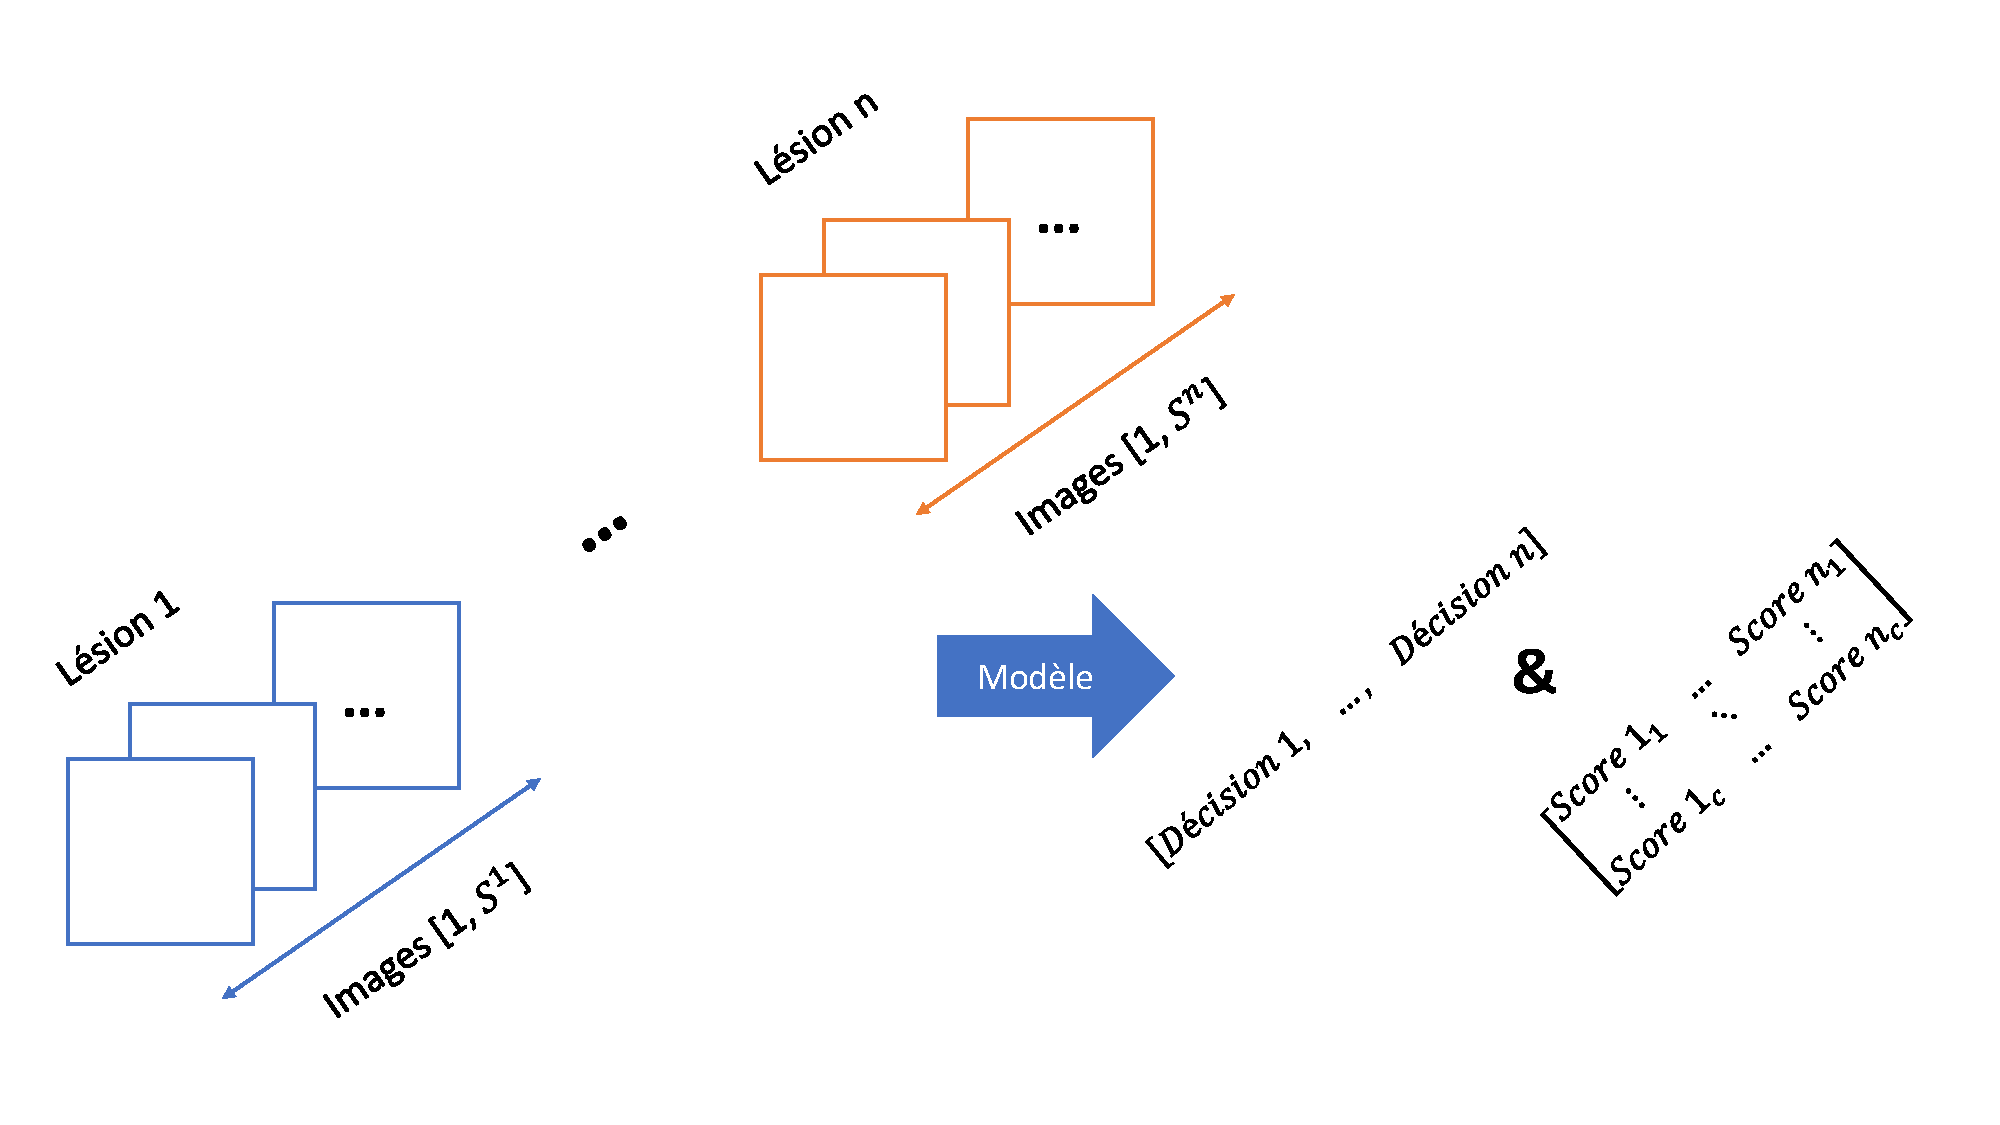
\includegraphics[width=0.65\linewidth]{contents/chapter_7/resources/scheme_patient_decision_objectives.pdf}
    \caption{Schéma récapitulatif de la problématique de l'inconsistance du nombres d'images constituant les lésions et de l'obtention de décisions et scores pour chacune de ces lésions.}
    \label{fig:scheme_patient_decision_objectives}
\end{figure}\par
\clearpage

\section{Approches supervisées}
\label{sec:patient_decision_supervised}
Cette section dédiée aux approches supervisées se consacre à des schémas d'apprentissages supervisés, c'est-à-dire dont la relation entre les instances et annotations est directe. Les données \gls{rcm} exploitées dans ce travail possèdent~:
\begin{inlinerate}
    \item d'une part des annotations à bas niveau ou \textbf{niveau image},
    \item d'autre part des annotations à haut niveau ou \textbf{niveau lésionnel}. 
\end{inlinerate} L'une des contraintes majeures associées à ces données est l'inconsistance du nombre d'images entre les lésions composant le jeu de données. Ainsi, une lésion peut comporter un nombre d'image compris entre une dizaine et une centaine d'entre elles. Il est donc nécessaire de gérer cette variabilité au sein du processus de classification mis en place.\par

Afin de résoudre cette tâche de manière supervisée, cette section propose un mécanisme de prédiction en deux temps~: 
\begin{itemize}
    \item une première étape de prédiction \textbf{au niveau image}, dont le but consiste à émettre une étiquette à chaque image,
    \item une seconde étape de prédiction \textbf{au niveau lésionnel} dont la finalité est d'évaluer la lésion à partir de l'information résultant du processus de classification au niveau image.
\end{itemize} À cette fin, les données d'entraînement sont divisées en deux parts~:
\begin{inlinerate}
    \item l'une d'entre elle à destination du processus de prédiction image,
    \item et l'autre à destination du processus décisionnel des lésions.
\end{inlinerate}
Cette séparation des données d'entraînement en deux sous-ensembles permet de contrer un sur-apprentissage du modèle de prédiction au niveau lésionnel, en évitant une prise de décision sur des images dont les attentes sont déjà connues. Le schéma global mis en oeuvre dans cette section est disponible sur la \Cref{fig:scheme_patient_decision}.\par

\begin{figure}[H]
    \centering
    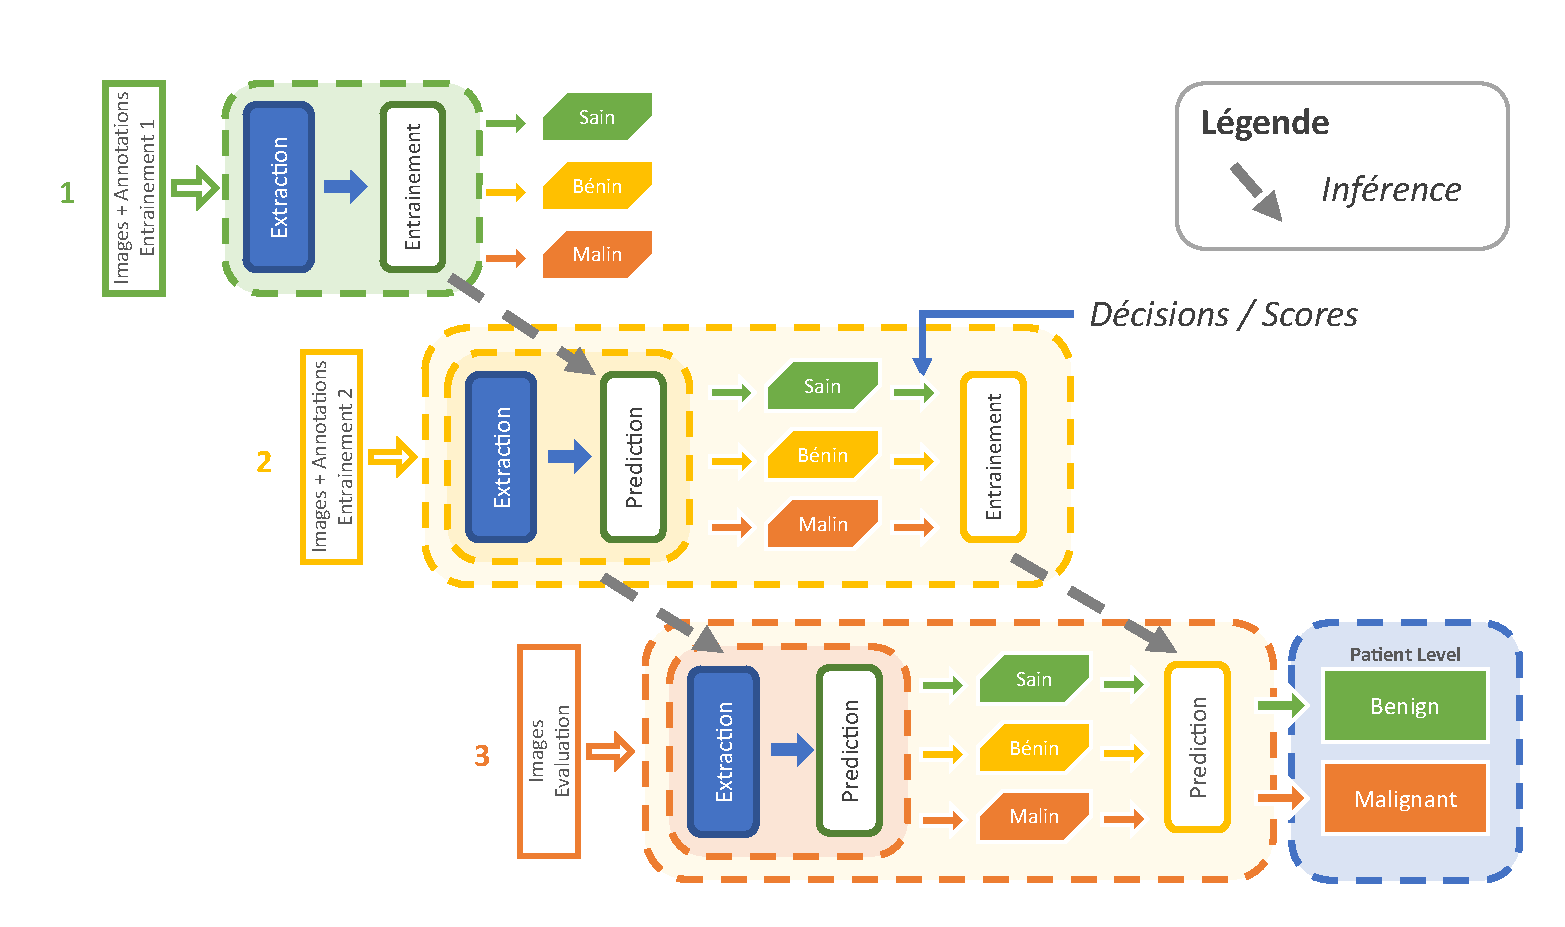
\includegraphics[width=0.95\linewidth]{contents/chapter_7/resources/scheme_patient_decision.pdf}
    \caption{Schéma de représentation du système complet de décision supervisée au niveau lésionnel. Le processus d'entraînement se subdivise en deux étapes~: une première étape d'entraînement du modèle de prédiction au niveau des instances images et une seconde étape permettant l'agrégation de l'information au niveau des lésions. La prédiction est ensuite réalisée sur les données de test par inférence des paramètres précédemment entraînés.}
    \label{fig:scheme_patient_decision}
\end{figure}\par

Ainsi, la \textbf{prédiction au niveau image} de ce processus exploite les méthodes issues des \Cref{chap:chapter_5,chap:chapter_6}, dont les expérimentations reposent sur la mise en place d'un processus de détection des images. Cette prédiction est assurée dans un premier temps par les méthodes d'extraction de caractéristiques jugées les plus pertinentes de ces parties, rappelées en \Cref{sec:patient_decision_methodology}. Ainsi, sont utilisées \textbf{des méthodes manuelles spatiales et fréquentielles} dont le nombre de caractéristiques extraites est de l'ordre de la dizaine, et \textbf{par transfert de connaissances sur des \gls{cnn}} pré-entraînés dont le nombre de caractéristiques dépasse la centaine. Dans un second temps, ces caractéristiques sont mises à l'échelle par \textbf{une normalisation de type Minimum / Maximum} puis séparées à l'aide d'\textbf{un modèle \gls{svm} à noyau linéaire}. Les hyperparamètres de ce dernier sont rappelés au niveau de la  \Cref{tab:parameters_lesion_classification_image_supervised}.\par

\begin{table}[H]
    \centering
    \begin{tabular}{lll}
        \toprule
        \textbf{Modèle}                                 & \textbf{Hyperparamètres}  & \textbf{Valeurs}                          \\ \midrule
        \gls{svm} - Noyau linéaire                      & C                         & [0,001, 0,01, 0,1, 1, 10, 100, 1000]      \\ 
        \bottomrule 
    \end{tabular} 
    \caption{Table reprenant le modèle et les hyperparamètres du modèle de classification employé pour la détection bas niveau des images.}
    \label{tab:parameters_lesion_classification_image_supervised}
\end{table}\par

La \textbf{prédiction au niveau des lésions} de ce processus tente d'établir une relation entre les diagnostics des images réalisés à l'aide de la première partie de ce processus et les annotations des lésions. Le nombre d'instances variant entre chaque lésion, les méthodes présentées ci-dessous sont mise au point pour supporter cette contrainte de fonctionnement. Ainsi, deux types potentiels de données d'entrée sont envisagés dans cette seconde partie de la classification, donnant lieu à deux types d'approches dont~:
\begin{itemize}
    \item   une approche au niveau des \textbf{décisions} de classification de la première étape, défini par l'ensemble $\mathbf{N}$. Ces données sont de la forme $instances \times 1$, dans lequel $instances$ est une variable propre à chaque lésion. Afin de réduire ces données à un vecteur commun, chaque classe est réduite par la relation $ratio_c = \dfrac{classe_c}{instances}$, aboutissant à un vecteur réel de dimension $1 \times classes$. À partir de ce vecteur, deux méthodes ont été définies, dont~:
            \begin{itemize}
                \item une méthode dite de \textbf{priorité} par laquelle est privilégiée la détection d'une classe hiérarchiquement supérieure comme décision globale à la lésion. Cette méthode est considéré sous le terme de \textbf{Décisions - Priorité}.
                \item une méthode dite par seuils \textbf{dynamiques} par laquelle des seuils optimaux sont déterminés pour chaque classe en privilégiant les classes prioritaires. Cette méthode est considéré sous le terme de \textbf{Décisions - Dynamique}.
            \end{itemize}
    \item   une approche au niveau des \textbf{scores} de classification de la première étape, défini par l'ensemble $\mathbf{R}$. Cette approche aboutit à un vecteur de taille $instances \times classes$, dans lequel $instances$ est une variable propre à chaque lésion et $classes$ est le nombre de classes prédites soit 2. Afin de réduire là encore ces données à un vecteur commun, chaque classe est réduite soit par une fonction de \textbf{moyenne} soit de \textbf{maximum} aboutissant à un vecteur réel de dimension $1 \times classes$. Puis, par seuil \textbf{dynamique} sur chacune des classes, des seuils optimaux sont définis en privilégiant les classes prioritaires. La combinaison de réduction par moyenne et seuil dynamique est considéré sous le terme de \textbf{Scores - Moyenne} et la combinaison de réduction par maximum et seuil dynamique est considéré sous le terme de  \textbf{Scores - Maximum}.
\end{itemize}\par
\clearpage

\section{Approches faiblement supervisées}
\label{sec:patient_decision_weak}
Une approche est décrite comme étant faiblement supervisée lorsque l'apprentissage de la relation entre les données et les annotations n'est pas directe. Ainsi, ces méthodes faiblement supervisées sont rassemblées en trois catégories majeures~\cite{Zhou2018}, dont~:
\begin{inlinerate}
    \item la \textbf{supervision dite incomplète} lorsque les données d'entraînement sont partiellement annotées,
    \item la \textbf{supervision dite inexacte} lorsque les annotations sont insuffisantes vis à vis du niveau de détails souhaité,
    \item et la \textbf{supervision dite imprécise} lorsque les annotations proviennent de sources manquant d'exactitude.
\end{inlinerate} Ces diverses approches ont notamment servi à la résolution de tâches telles que la catégorisation de textes~\cite{Andrews2003,Settles2008} ou d'images~\cite{Chen2004,Tang2009}. Plus spécifiquement au domaine médical, ces techniques ont permis l'aide au diagnostic d'images médicales sur des pathologies pulmonaires ou du colon~\cite{Dundar2007} mais également du cancer du sein~\cite{Sudharshan2019}.\par

À cette fin, les annotations et les données images propres à chacune des lésions sont employées pour servir cette tâche faiblement supervisée. Par la nature des données en notre possession, cette nouvelle section s'intéresse au second mode de supervision dite inexacte, par l'utilisation de \gls{mil}. De manière plus formelle ces techniques visent à résoudre la relation $f: X \mapsto Y$, à l'aide des données $D=\{(X_1,y_1),(X_2,y_2),\ldots,(X_b,y_b)\}$ avec $X=\{x_1,x_2,\ldots,x_b\}$ représentant un ensemble ou \textit{bag} d'information composé d'images et $y$ l'annotation associée~\cite{foulds2010}.\par

Ce principe de méthodes à instances multiples est initialement issu du domaine de la recherche de médicaments, domaine dans lequel sont recherchées des molécules ainsi que le ou les \textit{conformères} (comprendre les formes que peuvent adopter ces molécules) responsables d'une activité biologique~\cite{Dietterich1997}. Ainsi dans ce contexte, l'activité biologique observée (\textbf{annotation}) est associée à une molécule (\textbf{ensemble}) dont certains conformères (\textbf{instances}) sont responsables du phénomène observé. Ce faisant, la théorie de base des méthodes à instances multiples stipule qu'un ensemble dont l'annotation est négative ne possède aucune instance relative au phénomène observé, tandis qu'un ensemble dont l'annotation est positive contient au moins une instance relative au phénomène observé~\cite{Dietterich1997}.\par

Par cette idée, de nombreuses théories ont émergé étendant le principe de techniques supervisées (principes de régression logistique, d'arbre de décision, \ldots) à la théorie des instances multiples~\cite{Maron1998,Xu2004,Blockeel2005}. Devant ces nombreuses théories et suite aux travaux des \Cref{chap:chapter_5} et \Cref{chap:chapter_6} mettant en avant l'efficacité des \gls{svm} sur cette problématique d'images \gls{rcm}, ce manuscrit s'intéresse à leur extension au principe d'instances multiples. L'un de ces travaux~\cite{Doran2014} développe plusieurs de ces approches et met notamment en avant trois propriétés essentielles des \gls{svm}~:
\begin{inlinerate}
    \item la solidité,
    \item l'exhaustivité,
    \item et la convexité.
\end{inlinerate} Ces propriétés sont toutes intrinsèques aux \gls{svm} et ne peuvent être satisfaites par cette extension au principe d'instances multiples. Il est donc nécessaire de procéder à un compromis de ces propriétés~\cite{Doran2014}.\par

Le travail de ce chapitre n'approfondit pas ces diverses propriétés, en revanche les divers modes d'approches associés à l'implémentation de ce principe sont envisagés, dont~: 
\begin{itemize}
    \item des approches par \textbf{instances} dont la méthode consiste à déterminer un hyperplan directement à partir des instances, sans considérer les annotations au niveau des ensembles~\cite{Andrews2003}. La séparation des ensembles découle de l'application du principe de base de la théorie des instances multiples, dans laquelle un ensemble est considéré positif si au moins l'une des instances qui le compose est considérée positive.
    \item des approches par \textbf{ensembles} dont le principe repose sur les annotations des ensembles et consiste à opérer la séparation par hyperplan au niveau des ensembles à partir de noyaux d'ensembles~\cite{Gartner2002}.
    \item des approches dites \textbf{hybrides} dont le principe se situe à mi-chemin entre les deux précédentes méthodes~\cite{Bunescu2007}.
\end{itemize}\par 

Ainsi, ces divers modes d'approches sont considérés dans les prochains paragraphes de ce travail. Dans le but de ne pas évaluer l'ensemble de ces modèles, ce travail ne se focalise que sur ceux jugés de manière empirique comme les plus pertinents au niveau de la classification d'ensembles par l'étude de Doran et al.~\cite{Doran2014}. Dans un premier temps, le modèle \gls{misvm} évalué dans ce travail suit une approche par \textit{instances}, dont le principe réside sur l'estimation de la meilleur instance représentative de chaque ensemble puis procède à une classification par \gls{svm}~\cite{Andrews2003}. Dans un second temps, le modèle \gls{nsk} employé suit une approche par \textbf{ensembles}, dont le principe consiste à projeter chaque ensemble et ses instances dans un nouvel espace de caractéristiques sur lequel est réalisé la séparation par \gls{svm}~\cite{Gartner2002}. Enfin, le modèle \gls{sbmil} choisi suit un type d'approche dite \textbf{hybride}, dont le principe stipule que \textbf{les instances d'ensembles négatifs sont négatives} et \textbf{les instances d'ensembles positifs sont négatives ou positives} dont le balancement est géré par une variable inconnue et pour lequel la totalité des instances est projetée avant séparation par un modèle \gls{svm}~\cite{Bunescu2007}.\par

Dans le but d'évaluer la pertinence de ces diverses méthodes, ce chapitre se consacre à l'évaluation de chacune d'entre elles combinée aux représentants des trois catégories d'extraction de caractéristiques formulées lors du \Cref{chap:chapter_5} et rappelées lors de la \Cref{sec:patient_decision_methodology}. De plus, suite aux résultats démontrant l'importance de la normalisation lors du \Cref{chap:chapter_5}, l'impact de la normalisation par Minimum et Maximum est évalué en combinaison de ces modèles faiblement supervisés.\par

L'ensemble des modèles de prédiction exploitant le principe d'\gls{mil} mis en oeuvre dans ce chapitre sont listés en \Cref{tab:patient_decision_weak_hyperparameters}. Afin de mener à bien la réalisation de ces expériences, ce travail se repose essentiellement sur la librairie logicielle \textit{MISVM} prévue à cet effet~\cite{Doran2014}.\par

\begin{table}[H]
    \centering
    \begin{tabular}{lll}
    \toprule
    \textbf{Méthode}    & \textbf{Paramètre}& \textbf{Valeurs}                                  \\ \midrule
    \gls{misvm}         & \multirow{3}{*}{C}& \multirow{3}{*}{[0,01, 0,1, 1, 10, 100, 1000]}    \\ \cline{1-1}
    \gls{nsk}           &                   &                                                   \\ \cline{1-1} 
    \gls{sbmil}         &                   &                                                   \\ \bottomrule 
    \end{tabular}    
    \caption{Table reprenant les divers modèles utilisant le principe d'\gls{mil} pour réaliser une classification au niveau lésionnel, ainsi que leurs hyperparamètres associés.}
    \label{tab:patient_decision_weak_hyperparameters}
\end{table}\par
\clearpage

\section{Présentation des résultats}
Les précédentes sections de ce travail se sont consacrées à décrire des méthodes pour tenter de résoudre la problématique de prédiction au niveau des lésions à partir de données \gls{rcm}. Cette nouvelle section se dédie à la présentation des résultats pour donner suite aux diverses expérimentations mentionnées précédemment. Dans une première sous-section, le protocole d'expérimentation suivi pour permettre l'obtention des résultats est relaté et l'organisation de ces résultats est décrite. Puis dans une seconde sous-section, les divers résultats issus des expériences mentionnées précédemment sont développées.\par

\subsection{Protocole d'expérimentation}
Afin de réaliser l'évaluation de ces expériences, une \textbf{validation croisée imbriquée} est employée, déjà discutée lors de la \Cref{sec:models_settings}, pour ses avantages permettant ainsi l'obtention de métriques plus objectives sur les performances du système évalué~\cite{Cawley2010}. Ce type de structure de validation est plus robuste face au biais~\cite{Cawley2010} et est démontré empiriquement moins sensible au biais et à la variance lorsque celle-ci est couplée à des valeurs de $k$ comprises entre 5 et 10 pour l'évaluation~\cite{James2000}. La diversité de combinaisons relativement limitée de cette partie, permet à l'instar des précédents chapitres, d'obtenir des résultats dans un temps raisonnable malgré des valeur de $k$ élevées. Ainsi \textbf{une valeur de $k$ égale à 10} est utilisée pour l'évaluation, tandis qu'une valeur de 2 est conservée pour la boucle interne suffisante pour déterminer la meilleure combinaison d'hyperparamètres. Bien que considéré comme une possibilité, le schéma de validation de type \textit{leave-one-out} pour la boucle externe d'évaluation n'est pas utilisé car plus sujet à une variance élevée lors des mesures notamment en présence de valeurs aberrantes~\cite{Bengio2004}. De plus, un tel schéma de validation est bien plus coûteux à entreprendre puisqu'il nécessite autant de phases d'entraînement et d'évaluation, que d'instances dans le jeu de données considérée, soit 223 pour ce travail.\par

D'une part, pour procéder au mieux au réglage des paramètres des modèles précédents et, d'autre part, pour retenir une évaluation objective de ces processus malgré les déséquilibres d'annotations, il est nécessaire d'opter pour une métrique adaptée. Ces expériences emploient le \textbf{\fscore{}} permettant de représenter conjointement les mesures de précision et de rappel au sein d'une même métrique binaire. De plus, et afin de compléter l'analyse des résultats et de permettre un parallèle avec ceux des experts en dermatologie, les valeurs de \textbf{sensibilité} et de \textbf{spécificité} sont renseignées conjointement au \fscore{}. Comme pour l'article de Cinotti et al.~\cite{Cinotti2016}, ce processus décompose la présentation des résultats en deux temps. Dans un premier temps, est présentée l'analyse des mesures précédentes \textbf{sur l'ensemble des cas clinique} du jeu de données, en adoptant comme classe positive les annotations des lésions dites \textit{malignes}. Puis dans un second temps, les même mesures sont extraites \textbf{en ne considérant que les cas de \textbf{\gls{lm} et \gls{lmm}} parmi les annotations malignes} et en adoptant comme classe positive les annotations des lésions dites \textit{malignes}.\par

La partie dédiée aux résultats se décompose en diverses étapes, débutant dans un premier temps par une présentation des résultats obtenus \textbf{au niveau lésionnel par les diverses méthodes supervisées} présentée lors de la \Cref{sec:patient_decision_supervised}. Dans un second temps, ce travail procède à une présentation des résultats obtenus \textbf{au niveau lésionnel par l'utilisation des méthodes faiblement supervisées} listées lors de la \Cref{sec:patient_decision_weak}. En continuité de ces résultats sur les méthodes faiblement supervisées, ce travail procède à une analyse inversée par la méthode \gls{misvm}. Ainsi, ce travail évalue la qualité des prédictions au niveau des instances images, afin de déterminer la compréhension du phénomène à bas niveau par cette méthode.\par
\clearpage

\subsection{Résultats des expérimentations}
Dans cette section dédiée aux résultats, les diverses méthodes envisagées pour la prise de décision au niveau des lésions vont être traitées à l'aide de paragraphes respectifs. Cette première analyse à destination des méthodes supervisées se consacre aux résultats obtenus par ces diverses méthodes. Pour les méthodes spatiales, un \fscore{} de 0,80 associé à un écart-type de 0,11 est obtenu à l'aide de la méthode \textbf{Décisions - Priorité}~;~Pour les méthodes fréquentielles, un \fscore{} de 0,83 associé à un écart-type de 0,07 est obtenu à l'aide de la méthode \textbf{Décisions - Dynamique}~;~Enfin, pour les méthodes de transfert de connaissances, un \fscore{} de 0,89 associé à un écart-type de 0,08 est obtenu à l'aide de la méthode \textbf{Scores - Moyenne}. Ainsi, des différences significatives sont à remarquer entre les méthodes spatiales, fréquentielles et de transfert de connaissances, nettement à l'avantage de cette dernière méthode comme mise en avant lors du \Cref{chap:chapter_5}. L'utilisation du transfert de connaissances comme base d'extraction de caractéristiques et la méthode \textbf{Scores - Moyenne} permettent l'obtention d'une valeur de \textit{sensibilité} de 0,95 et de \textit{spécificité} de 0,70, Ces résultats peuvent être visualisés dans la \Cref{tab:results_lesion_classification_supervised_patient}.\par

\begin{table}[H]
    \centering
    \begin{tabular}{cllll}
        \toprule
        \multicolumn{1}{l}{}         &                              & Sensibilité               & Spécificité               & \Fscore{}                 \\ \midrule
        \multirow{4}{*}{Spatial}     & Décisions - Priorité         & \textbf{0,92$\pm$0,09}    & \textbf{0,40$\pm$0,16}    & \textbf{0,80$\pm$0,11}    \\
                                     & Décisions - Dynamique        & 0,80$\pm$0,19             & 0,66$\pm$0,22             & 0,80$\pm$0,13             \\
                                     & Scores - Maximum             & 0,83$\pm$0,18             & 0,57$\pm$0,25             & 0,79$\pm$0,12             \\
                                     & Scores - Moyenne             & 0,83$\pm$0,20             & 0,58$\pm$0,30             & 0,79$\pm$0,13             \\ \midrule
        \multirow{4}{*}{Fréquentiel} & Décisions - Priorité         & 0,93$\pm$0,06             & 0,37$\pm$0,25             & 0,80$\pm$0,11             \\
                                     & Décisions - Dynamique        & \textbf{0,82$\pm$0,08}    & \textbf{0,77$\pm$0,10}    & \textbf{0,83$\pm$0,07}    \\
                                     & Scores - Maximum             & 0,84$\pm$0,09             & 0,58$\pm$0,22             & 0,80$\pm$0,09             \\
                                     & Scores - Moyenne             & 0,80$\pm$0,14             & 0,72$\pm$0,25             & 0,81$\pm$0,09             \\ \midrule
        \multirow{4}{*}{Transfert}   & Décisions - Priorité         & 0,98$\pm$0,04             & 0,34$\pm$0,14             & 0,82$\pm$0,06             \\
                                     & Décisions - Dynamique        & 0,91$\pm$0,13             & 0,71$\pm$0,24             & 0,87$\pm$0,09             \\
                                     & Scores - Maximum             & 0,92$\pm$0,15             & 0,57$\pm$0,21             & 0,84$\pm$0,12             \\
                                     & Scores - Moyenne             & \textbf{0,95$\pm$0,09}    & \textbf{0,70$\pm$0,22}    & \textbf{0,89$\pm$0,08}    \\ \bottomrule
    \end{tabular}
    \caption{Table de résultats issus des processus de classification supervisée employés pour mener une classification au niveau lésionnel, exprimés selon la sensibilité, la spécificité et le \fscore{}.}
    \label{tab:results_lesion_classification_supervised_patient}
\end{table}

Ce second paragraphe se focalise sur les cas de lésions de types \gls{lm} et \gls{lmm} par ces mêmes méthodes de prédiction supervisées. Pour les méthodes spatiales, un \fscore{} de 0,80 associé à un écart-type de 0,14 est obtenu à l'aide de la méthode \textbf{Décisions - Dynamique}~;~Pour les méthodes fréquentielles, un \fscore{} de 0,83 associé à un écart-type de 0,09 est obtenu à l'aide de la méthode \textbf{Décisions - Dynamique}~;~Pour les méthodes de transfert de connaissances, un \fscore{} de 0,87 associé à un écart-type de 0,11 est obtenu à l'aide de la méthode \textbf{Scores - Moyenne}. À nouveau, des différences significatives sont à remarquer entre les méthodes spatiales, fréquentielles et de transfert de connaissances, à l'avantage de cette dernière méthode comme mise en avant lors du \Cref{chap:chapter_5}. La mise en oeuvre du transfert de connaissances comme base d'extraction de caractéristiques et la méthode \textbf{Scores - Moyenne} permettent l'obtention de résultats équivalents avec une valeur de \textit{sensibilité} de 0,95 et de \textit{spécificité} de 0,70 sur les lésions de types \gls{lm} et \gls{lmm}. Les diverses valeurs peuvent être visualisés sur la \Cref{tab:results_lesion_classification_supervised_patient_lm}.\par

\begin{table}[H]
    \centering
    \begin{tabular}{cllll}
        \toprule
        \multicolumn{1}{l}{}         &                              & Sensibilité               & Spécificité               & \Fscore{}                 \\ \midrule
        \multirow{4}{*}{Spatial}     & Décisions - Priorité         & 0,93$\pm$0,11             & 0,40$\pm$0,16             & 0,78$\pm$0,13             \\
                                     & Décisions - Dynamique        & \textbf{0,84$\pm$0,18}    & \textbf{0,66$\pm$0,22}    & \textbf{0,80$\pm$0,14}    \\
                                     & Scores - Maximum             & 0,83$\pm$0,18             & 0,57$\pm$0,25             & 0,77$\pm$0,14             \\
                                     & Scores - Moyenne             & 0,86$\pm$0,18             & 0,58$\pm$0,30             & 0,79$\pm$0,14             \\ \midrule
        \multirow{4}{*}{Fréquentiel} & Décisions - Priorité         & 0,93$\pm$0,07             & 0,37$\pm$0,25             & 0,77$\pm$0,13             \\
                                     & Décisions - Dynamique        & \textbf{0,84$\pm$0,12}    & \textbf{0,77$\pm$0,10}    & \textbf{0,83$\pm$0,09}    \\
                                     & Scores - Maximum             & 0,87$\pm$0,09             & 0,58$\pm$0,22             & 0,80$\pm$0,11             \\
                                     & Scores - Moyenne             & 0,82$\pm$0,14             & 0,72$\pm$0,25             & 0,81$\pm$0,12             \\ \midrule
        \multirow{4}{*}{Transfert}   & Décisions - Priorité         & 0,97$\pm$0,05             & 0,34$\pm$0,14             & 0,79$\pm$0,07             \\
                                     & Décisions - Dynamique        & 0,91$\pm$0,16             & 0,71$\pm$0,24             & 0,86$\pm$0,12             \\
                                     & Scores - Maximum             & 0,90$\pm$0,18             & 0,57$\pm$0,21             & 0,81$\pm$0,16             \\
                                     & Scores - Moyenne             & \textbf{0,95$\pm$0,11}    & \textbf{0,70$\pm$0,22}    & \textbf{0,87$\pm$0,11}    \\ \bottomrule
    \end{tabular}
    \caption{Table de résultats issus des processus de classification supervisée employés pour mener une classification au niveau lésionnel sur les pathologies de \gls{lm} et \gls{lmm}, exprimés selon la sensibilité, la spécificité et le \fscore{}.}
    \label{tab:results_lesion_classification_supervised_patient_lm}
\end{table}

\vspace{25pt}

\begin{table}[H]
    \centering
    \begin{tabular}{cllll}
        \toprule
        \multicolumn{1}{l}{}         &                      & Sensibilité               & Spécificité               & \Fscore{}                 \\ \midrule
        \multirow{6}{*}{Spatial}     & \gls{misvm}          & 0,69$\pm$0,13             & 0,57$\pm$0,22             & 0,70$\pm$0,12             \\
                                     & \gls{nsk}            & \textbf{0,81$\pm$0,12}    & \textbf{0,70$\pm$0,12}    & \textbf{0,81$\pm$0,08}    \\
                                     & \gls{sbmil}          & 0,10$\pm$0,08             & 0,99$\pm$0,06             & 0,18$\pm$0,13             \\
                                     & MMS + \gls{misvm}    & 0,78$\pm$0,14             & 0,77$\pm$0,14             & 0,81$\pm$0,12             \\
                                     & MMS + \gls{nsk}      & 0,78$\pm$0,11             & 0,69$\pm$0,13             & 0,79$\pm$0,08             \\
                                     & MMS + \gls{sbmil}    & 0,88$\pm$0,30             & 0,07$\pm$0,30             & 0,72$\pm$0,24             \\ \midrule
        \multirow{6}{*}{Fréquentiel} & \gls{misvm}          & 0,72$\pm$0,19             & 0,62$\pm$0,26             & 0,73$\pm$0,16             \\
                                     & \gls{nsk}            & 0,78$\pm$0,15             & 0,59$\pm$0,21             & 0,77$\pm$0,12             \\
                                     & \gls{sbmil}          & 0,27$\pm$0,28             & 0,84$\pm$0,29             & 0,39$\pm$0,23             \\
                                     & MMS + \gls{misvm}    & \textbf{0,83$\pm$0,12}    & \textbf{0,69$\pm$0,16}    & \textbf{0,82$\pm$0,10}    \\
                                     & MMS + \gls{nsk}      & 0,80$\pm$0,14             & 0,71$\pm$0,09             & 0,81$\pm$0,11             \\
                                     & MMS + \gls{sbmil}    & 0,09$\pm$0,06             & 1.00$\pm$0,00             & 0,16$\pm$0,09             \\ \midrule
        \multirow{6}{*}{Transfert}   & \gls{misvm}          & 0,83$\pm$0,12             & 0,76$\pm$0,17             & 0,84$\pm$0,10             \\
                                     & \gls{nsk}            & \textbf{0,86$\pm$0,10}    & \textbf{0,77$\pm$0,19}    & \textbf{0,86$\pm$0,11}    \\
                                     & \gls{sbmil}          & 0,17$\pm$0,11             & 0,90$\pm$0,09             & 0,28$\pm$0,15             \\
                                     & MMS + \gls{misvm}    & 0,83$\pm$0,10             & 0,77$\pm$0,16             & 0,84$\pm$0,07             \\
                                     & MMS + \gls{nsk}      & 0,86$\pm$0,10             & 0,72$\pm$0,19             & 0,85$\pm$0,09             \\
                                     & MMS + \gls{sbmil}    & 0,21$\pm$0,12             & 0,91$\pm$0,10             & 0,33$\pm$0,17             \\ \bottomrule
    \end{tabular}
    \caption{Table de résultats issus des processus de classification faiblement supervisée par \gls{mil} employés pour mener une classification au niveau lésionnel, exprimés selon la sensibilité, la spécificité et le \fscore{}.}
    \label{tab:results_lesion_classification_weakly_patient}
\end{table}
\clearpage

Cette seconde partie à destination des méthodes faiblement supervisées par \gls{mil} va permettre de décrire les résultats obtenus par ces diverses méthodes. Pour les méthodes spatiales, un \fscore{} de 0,81 associé à un écart-type de 0,08 est obtenu à l'aide de la méthode \textbf{\gls{nsk}}~;~Pour les méthodes fréquentielles, un \fscore{} de 0,82 associé à un écart-type de 0,10 est obtenu à l'aide de la méthode combinant \textbf{normalisation par Minimum / Maximum et \gls{misvm}}~;~Pour les méthodes de transfert de connaissances, un \fscore{} de 0,86 associé à un écart-type de 0,11 est obtenu à l'aide de la méthode \textbf{\gls{nsk}}. Ainsi, de même que pour les méthode supervisées, des différences significatives sont à remarquer entre les méthodes spatiales, fréquentielles et de transfert de connaissances. Cette dernière méthode comme base d'extraction de caractéristiques et la méthode \gls{nsk} permettent l'obtention d'une valeur de \textit{sensibilité} de 0,86 et de \textit{spécificité} de 0,77. Les valeurs détaillées des résultats d'expérimentation de techniques faiblement supervisées par \gls{mil} peuvent être visualisés sur la \Cref{tab:results_lesion_classification_weakly_patient}.\par

Ce second paragraphe à l'intention des méthodes faiblement supervisées par \gls{mil} se focalise sur les cas de \gls{lm} et \gls{lmm}. Pour les méthodes spatiales, un \fscore{} de 0,80 associé à un écart-type de 0,11 est obtenu à l'aide de la méthode \textbf{\gls{nsk}}~;~Pour les méthodes fréquentielles, un \fscore{} de 0,80 associé à un écart-type de 0,11 est obtenu à l'aide de la méthode combinant \textbf{normalisation par Minimum / Maximum au modèle \gls{nsk}}~;~Pour les méthodes de transfert de connaissances, un \fscore{} de 0,85 associé à un écart-type de 0,13 est obtenu par la méthode \textbf{\gls{nsk}}. À nouveau, la méthode d'extraction par transfert de connaissances permet l'obtention des résultats les plus pertinents en combinaison de la méthode \gls{nsk}, soit des valeurs de \textit{sensibilité} de 0,87 et de \textit{spécificité} de 0,77. Ces nouvelles valeurs liées à l'évaluation des méthodes faiblement supervisées sur les cas de \gls{lm} et \gls{lmm} peuvent être visualisés sur la \Cref{tab:results_lesion_classification_weakly_patient_lm}.\par

\begin{table}[H]
    \centering
    \begin{tabular}{cllll}
        \toprule
        \multicolumn{1}{l}{}         &                          & Sensibilité               & Spécificité               & \Fscore{}                 \\ \midrule
        \multirow{6}{*}{Spatial}     & \gls{misvm}              & 0,69$\pm$0,17             & 0,57$\pm$0,22             & 0,69$\pm$0,14             \\
                                     & \gls{nsk}                & \textbf{0,82$\pm$0,15}    & \textbf{0,70$\pm$0,12}    & \textbf{0,80$\pm$0,11}    \\
                                     & \gls{sbmil}              & 0,11$\pm$0,09             & 0,99$\pm$0,06             & 0,20$\pm$0,14             \\
                                     & MMS + \gls{misvm}        & 0,78$\pm$0,17             & 0,77$\pm$0,14             & 0,80$\pm$0,16             \\
                                     & MMS + \gls{nsk}          & 0,81$\pm$0,14             & 0,69$\pm$0,13             & 0,79$\pm$0,09             \\
                                     & MMS + \gls{sbmil}        & 0,86$\pm$0,30             & 0,07$\pm$0,30             & 0,67$\pm$0,23             \\ \midrule
        \multirow{6}{*}{Fréquentiel} & \gls{misvm}              & 0,71$\pm$0,21             & 0,62$\pm$0,26             & 0,71$\pm$0,19             \\
                                     & \gls{nsk}                & 0,78$\pm$0,12             & 0,59$\pm$0,21             & 0,75$\pm$0,10             \\
                                     & \gls{sbmil}              & 0,25$\pm$0,28             & 0,84$\pm$0,29             & 0,37$\pm$0,22             \\
                                     & MMS + \gls{misvm}        & 0,82$\pm$0,13             & 0,69$\pm$0,16             & 0,80$\pm$0,12             \\
                                     & MMS + \gls{nsk}          & \textbf{0,82$\pm$0,14}    & \textbf{0,71$\pm$0,09}    & \textbf{0,80$\pm$0,11}    \\
                                     & MMS + \gls{sbmil}        & 0,11$\pm$0,06             & 1.00$\pm$0,00             & 0,19$\pm$0,10             \\ \midrule
        \multirow{6}{*}{Transfert}   & \gls{misvm}              & 0,82$\pm$0,13             & 0,76$\pm$0,17             & 0,82$\pm$0,12             \\
                                     & \gls{nsk}                & \textbf{0,87$\pm$0,09}    & \textbf{0,77$\pm$0,19}    & \textbf{0,85$\pm$0,13}    \\
                                     & \gls{sbmil}              & 0,19$\pm$0,10             & 0,90$\pm$0,09             & 0,30$\pm$0,15             \\
                                     & MMS + \gls{misvm}        & 0,85$\pm$0,10             & 0,77$\pm$0,16             & 0,84$\pm$0,08             \\
                                     & MMS + \gls{nsk}          & 0,88$\pm$0,10             & 0,72$\pm$0,19             & 0,84$\pm$0,11             \\
                                     & MMS + \gls{sbmil}        & 0,25$\pm$0,13             & 0,91$\pm$0,10             & 0,38$\pm$0,18             \\ \bottomrule
    \end{tabular}
    \caption{Table de résultats issus des processus de classification faiblement supervisée par \gls{mil} employés pour mener une classification au niveau lésionnel sur les pathologies de \gls{lm} et \gls{lmm}, exprimés selon la sensibilité, la spécificité et le \fscore{}.}
    \label{tab:results_lesion_classification_weakly_patient_lm}
\end{table}

Pour finir, ce paragraphe se consacre à la présentation des courbes \gls{roc} au niveau lésionnel des divers méthodes mentionnées précédemment. Sur l'ensemble des cas cliniques, la méthode supervisée issue du modèle de prédiction \textbf{Scores - Moyenne} permet l'obtention d'un score \gls{auc} de 0,87~;~la méthode faiblement supervisée par utilisation du modèle \textbf{\gls{nsk}} permet quant à elle l'obtention d'un score \gls{auc} de 0,83. Sur les seuls cas de \gls{lm} et \gls{lmm}, la méthode supervisée issue du modèle de prédiction \textbf{Scores - Moyenne} permet l'obtention d'un score \gls{auc} similaire de 0,88~;~la méthode faiblement supervisée par utilisation du modèle \textbf{\gls{nsk}} permet quant à elle l'obtention d'un score \gls{auc} de 0,83 identique à celui sur l'ensemble des lésions. L'ensemble de ces courbes \gls{roc} et de ces scores \gls{auc} peuvent être visualisées sur la \Cref{fig:results_lesion_roc_lesions}.\par

\begin{figure}[H]
    \centering
    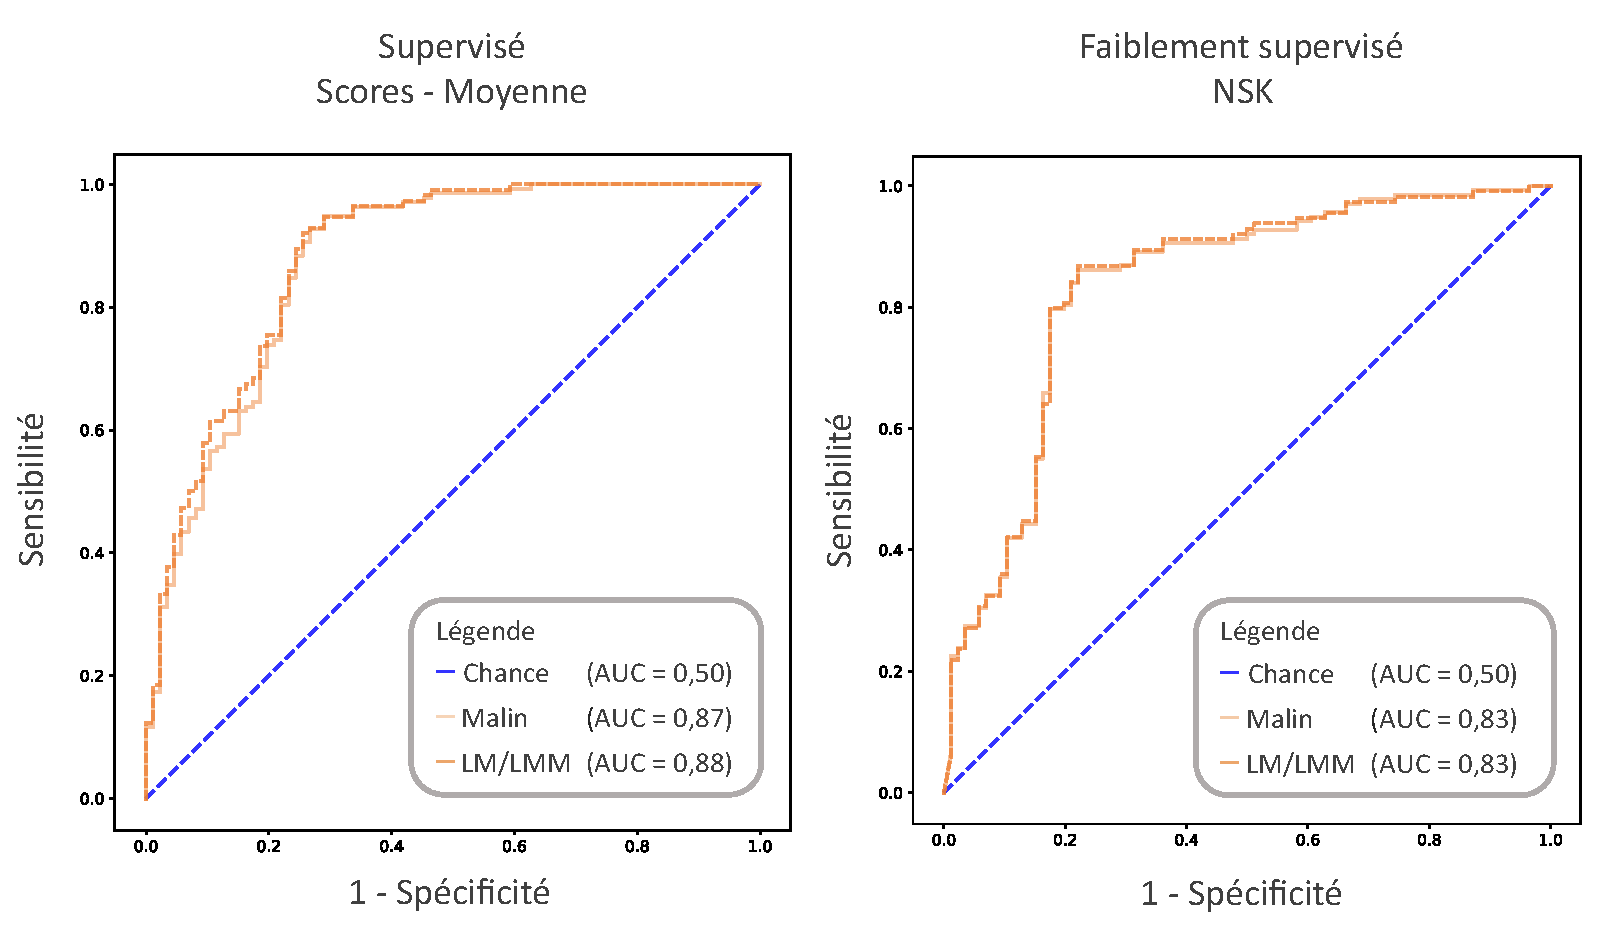
\includegraphics[width=\linewidth]{contents/chapter_7/resources/results_lesion_roc_lesions.pdf}
    \caption{Courbes \gls{roc} issues des résultats de la prédiction au niveau des lésions sur l'ensemble des cas, figurant à l'aide d'un trait orange estompé tracé en continu, mais également sur les cas de \gls{lm} et \gls{lmm}, figurant à l'aide d'un trait orange tracé en pointillés. À gauche, les courbes issues des prédictions employant la méthode \textit{Scores - Moyenne}~;~À droite, les courbes issues des prédictions du modèle \textit{\gls{nsk}}.}
    \label{fig:results_lesion_roc_lesions}
\end{figure}\par

Cette dernière partie se dédie aux résultats de prédiction des méthodes faiblement supervisées par \gls{mil} dont l'approche se base sur les instances et permet de revenir à un niveau de prédiction sur les instances. À cet effet, seul le modèle \textbf{\gls{misvm}} permet de revenir à un tel niveau de prédiction au sein de ce travail. Pour les méthodes spatiales, un \fscore{} de 0,56 associé à un écart-type de 0,14 est obtenu par combinaison de la \textbf{normalisation Minimum / Maximum et du modèle \gls{misvm}}~;~Pour les méthodes fréquentielles, un \fscore{} de 0,59 associé à un écart-type de 0,15 est obtenu par combinaison de la \textbf{normalisation Minimum / Maximum et du modèle \gls{misvm}}~;~Pour les méthodes de transfert de connaissances, un \fscore{} de 0,64 associé à un écart-type de 0,16 est obtenu avec le modèle \textbf{\gls{misvm}} seul. Les résultats de cette prédiction au niveau des instances images sont visibles dans la \Cref{tab:results_lesion_classification_weakly_image}.\par

\begin{table}[H]
    \centering
    \begin{tabular}{cllll}
        \toprule
        \multicolumn{1}{l}{}         &                      & Sensibilité               & Spécificité               & \Fscore{}                 \\ \midrule
        \multirow{2}{*}{Spatial}     & \gls{misvm}          & 0,29$\pm$0,13             & 0,90$\pm$0,08             & 0,42$\pm$0,14             \\
                                     & MMS + \gls{misvm}    & \textbf{0,42$\pm$0,15}    & \textbf{0,93$\pm$0,05}    & \textbf{0,56$\pm$0,14}    \\ \midrule
        \multirow{2}{*}{Fréquentiel} & \gls{misvm}          & 0,29$\pm$0,22             & 0,89$\pm$0,28             & 0,42$\pm$0,20             \\
                                     & MMS + \gls{misvm}    & \textbf{0,45$\pm$0,15}    & \textbf{0,93$\pm$0,05}    & \textbf{0,59$\pm$0,15}    \\ \midrule
        \multirow{2}{*}{Transfert}   & \gls{misvm}          & \textbf{0,48$\pm$0,16}    & \textbf{0,97$\pm$0,02}    & \textbf{0,64$\pm$0,16}    \\
                                     & MMS + \gls{misvm}    & 0,42$\pm$0,14             & 0,97$\pm$0,02             & 0,57$\pm$0,14             \\ \bottomrule
    \end{tabular}
    \caption{Table de résultats issus de l'application du modèle \gls{misvm} employé pour mener une classification au niveau des instances, sur l'ensemble des images annotées, et exprimés selon la sensibilité, la spécificité et le \fscore{}.}
    \label{tab:results_lesion_classification_weakly_image}
\end{table}

Ce second paragraphe reprend les résultats de prédiction des méthodes faiblement supervisées par \gls{mil} sur les images issues de lésions de type \gls{lm} et \gls{lmm}. Pour les méthodes spatiales, un \fscore{} de 0,60 associé à un écart-type de 0,14 est obtenu par combinaison de la \textbf{normalisation Minimum / Maximum et du modèle \gls{misvm}}~;~Pour les méthodes fréquentielles, un \fscore{} de 0,62 associé à un écart-type de 0,14 est obtenu par combinaison de la \textbf{normalisation Minimum / Maximum et du modèle \gls{misvm}}~;~Pour les méthodes de transfert de connaissances, un \fscore{} de 0,65 associé à un écart-type de 0,16 est obtenu avec le modèle \textbf{\gls{misvm}} seul. Le détail de ces résultats de prédiction au niveau des instances images à partir des méthodes \gls{mil} est disponible dans la \Cref{tab:results_lesion_classification_weakly_image_lm}.\par

\begin{table}[H]
    \centering
    \begin{tabular}{cllll}
        \toprule
        \multicolumn{1}{l}{}         &                      & Sensibilité               & Spécificité               & \Fscore{}                 \\ \midrule
        \multirow{2}{*}{Spatial}     & \gls{misvm}          & 0,31$\pm$0,16             & 0,84$\pm$0,19             & 0,46$\pm$0,18             \\
                                     & MMS + \gls{misvm}    & \textbf{0,44$\pm$0,14}    & \textbf{0,89$\pm$0,18}    & \textbf{0,60$\pm$0,14}    \\ \midrule
        \multirow{2}{*}{Fréquentiel} & \gls{misvm}          & 0,28$\pm$0,23             & 0,87$\pm$0,32             & 0,42$\pm$0,24             \\
                                     & MMS + \gls{misvm}    & \textbf{0,47$\pm$0,15}    & \textbf{0,86$\pm$0,25}    & \textbf{0,62$\pm$0,14}    \\ \midrule
        \multirow{2}{*}{Transfert}   & \gls{misvm}          & \textbf{0,49$\pm$0,16}    & \textbf{0,94$\pm$0,07}    & \textbf{0,65$\pm$0,16}    \\
                                     & MMS + \gls{misvm}    & 0,43$\pm$0,16             & 0,94$\pm$0,08             & 0,59$\pm$0,17             \\ \bottomrule
    \end{tabular}
    \caption{Table de résultats issus de l'application du modèle \gls{misvm} employés pour mener une classification au niveau des instances, sur les images annotées issues de pathologies de \gls{lm} et \gls{lmm}, et exprimés selon la sensibilité, la spécificité et le \fscore{}.}
    \label{tab:results_lesion_classification_weakly_image_lm}
\end{table}

Pour finir cette présentation des résultats de prédiction au niveau des images à partir de méthodes faiblement supervisées employant le principe de \gls{mil}, ce paragraphe présente les résultats des courbes \gls{roc} et \gls{auc}. Ainsi sur l'ensemble des cas cliniques, \textbf{la méthode \gls{misvm}} permet l'obtention d'un score \gls{auc} de 0,87. Cette même méthode, focalisée sur les cas de \gls{lm} et \gls{lmm}, permet l'obtention d'un score \gls{auc} de 0,82. Les courbes \gls{roc} et les scores \gls{auc} obtenues à partir de la prédiction sur des instances images peuvent être visualisées sur la \Cref{fig:results_lesion_roc_instances}.\par

\begin{figure}[H]
    \centering
    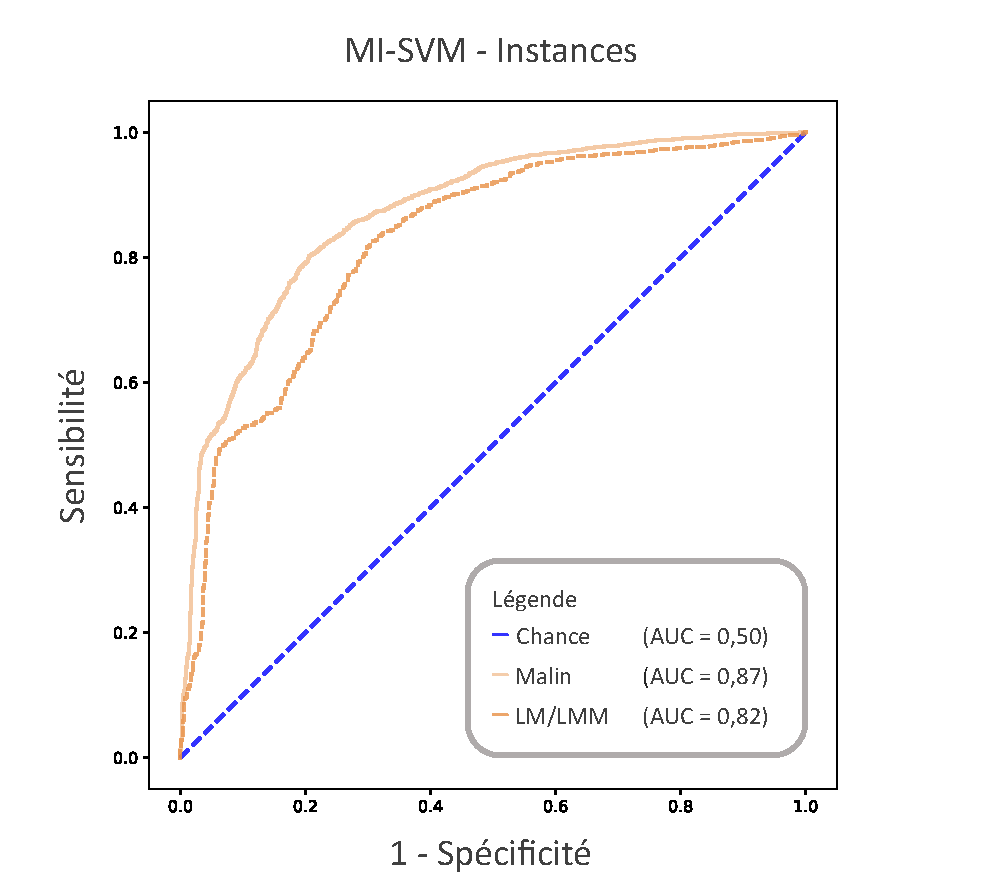
\includegraphics[width=0.7\linewidth]{contents/chapter_7/resources/results_lesion_roc_instances.pdf}
    \caption{Courbes \gls{roc} issues de la prédiction au niveau des instances sur l'ensemble des cas, figurant à l'aide d'un trait orange estompé tracé en continu, et en ne considérant que les cas de \gls{lm} et \gls{lmm} parmi les annotations malignes, figurant à l'aide d'un trait orange tracé en pointillés. Les courbes sont issues  du mode de prédiction faiblement supervisée sur la base de la théorie \gls{mil} par utilisation du modèle \gls{misvm}.}
    \label{fig:results_lesion_roc_instances}
\end{figure}\par

\section{Discussion}
Cette partie de discussion se dédie à l'analyse des résultats de la précédente section. Ce premier paragraphe détaille les observations issues des méthodes de prédiction supervisées au niveau lésionnel. Les \fscore{} sont pour la plupart homogènes si l'on considère chaque méthode d'extraction indépendamment, mais les mesures de sensibilité et spécificité propres à chacune varient fortement entre méthodes. Ainsi, la méthode de \textbf{Décisions - Priorité} bénéficie d'une forte sensibilité liée à son principe privilégiant la moindre détection de la classe prioritaire / positive, mais se contente d'une faible spécificité. Ce principe est ainsi plus nuancé par la méthode \textbf{Décisions - Dynamique} qui apporte un seuil dynamique d'activation, et dont résultent des valeurs de sensibilité et spécificité plus équilibrés et supérieure en terme de \fscore{}. Néanmoins, cette méthode nécessite de laisser de côté certaines détections jusqu'à atteindre un certain seuil d'activation ; ce principe peux être difficile à utiliser en milieu clinique. Afin de modérer ces deux méthodes, ont été proposées deux approches par scores. La première de ces méthodes \textbf{Scores - Maximum} initialement conçue pour conserver la sensibilité de la méthode \textbf{Décisions - Priorité}, perd une forte partie de celle-ci mais améliore nettement sa spécificité. La seconde de ces méthodes \textbf{Scores - Moyenne} initialement conçue pour affiner la décision de la méthode \textbf{Décisions - Dynamique}, restes-en deçà de celle-ci avec néanmoins un score important sur les caractéristiques issues de l'extraction par transfert de connaissances. En ce qui concerne les résultats sur les pathologies malignes toutes confondues et sur les cas de \gls{lm} et \gls{lmm}, peu de différences sont à remarquer entre ces deux situations, ces méthodes semblent ainsi robustes au type de pathologie traitée.\par
\clearpage

Ce second paragraphe propose une analyse des méthodes faiblement supervisées par \gls{mil} dont les résultats sont très hétérogènes, par contraste aux méthodes supervisées. Ainsi, ce paragraphe procède à une analyse méthode par méthode. Dans un premier temps, \textbf{le modèle \gls{misvm}} permet l'obtention de modèle modèles plus sensibles que spécifiques et dont le score global semble assez dépendant du type d'extraction employée, les résultats étant maximisés par l'utilisation du transfert de connaissances. Néanmoins, l'utilisation d'une \textbf{normalisation par Minimum / Maximum} semble bénéfique dans la plupart des situations et contribue à baisser cette dépendance à la méthode d'extraction de caractéristiques. Dans un second temps, \textbf{le modèle \gls{nsk}} est choisie pour représenter la catégorie des approches par noyaux d'ensembles, et semble être la méthode la plus adaptée dans ce schéma faiblement supervisé avec le jeu de données en notre possession. Ainsi, cette méthode apporte des résultats assez proches quel que soit le mode d'extraction de caractéristiques choisi, et possède une bonne sensibilité bien que les valeurs de spécificité soient assez proches. Dans un dernier temps, \textbf{le modèle \gls{sbmil}} est utilisée comme représentante des approches hybride, non concluante dans ce cadre. En effet, ces méthodes ont une grande spécificité mais une sensibilité quasi-inexistante. Pour finir, les conclusions qui régissent les résultats sur les pathologies malignes toutes confondues et sur les cas de \gls{lm} et \gls{lmm} sont similaires à celle des méthodes supervisées ; ces méthodes semblent ainsi robustes au type de pathologie traitée.\par

Ainsi, les deux approches proposées, c'est à dire par entraînement supervisé et faiblement supervisée, sont adaptées à la problématique actuelle bien que l'approche supervisé soit sensiblement supérieure. Cette supériorité des méthodes supervisée se traduit notamment sur les valeurs \gls{auc} avec des valeurs de 0,87 pour \textbf{le modèle Scores - Moyenne} et de 0,83 pour \textbf{le modèle \gls{nsk}}. Il est à remarquer que toutes ces approches possèdent un écart-type assez élevé situé entre 0,08 et 0,15, à l'exception de \textbf{la méthode \gls{sbmil}} dont les valeurs sont encore plus conséquentes. Cette tendance assez forte montre une certaine dépendance aux données mais peut être la conséquence du nombre restreint d'échantillons au niveau lésionnel du jeu de données, soit 223 lésions. Un élément supplémentaire à considérer est la complexité nécessaire à l'obtention des résultats supervisés, dont le nombre de paramètres est supérieur aux méthodes faiblement supervisées présentées. Par ailleurs, les méthodes supervisées utilisées ici nécessitent un processus en deux temps (voir trois si l'on considère l'extraction de caractéristiques), tandis que les méthodes faiblement supervisées nécessitent une étape de moins. Le dernier argument en faveur des méthodes faiblement supervisées est celui de la très faible quantité d'annotations sollicitée pour parvenir à de tel résultats, soit 223 annotations.\par

Afin de mesurer, d'une part la compréhension au niveau lésionnel de ces modèles faiblement supervisés et d'autre part d'évaluer la qualité d'un système permettant de revenir à des prédiction bas niveau, une évaluation des prédiction au niveau des instance à été réalisée. Ces tests sont menés sur \textbf{le modèle \gls{misvm}}, et on permis d'obtenir une valeur de \fscore{} de 0,64 et \gls{auc} de 0,87 sur l'ensemble des cas cliniques. Cette valeur était en comparaison respectivement à un \fscore{} de 0,82 et \gls{auc} au 0,90 sein du \Cref{chap:chapter_5} avec des valeurs d'écart-type beaucoup plus restreintes. Il existe de ce fait une différence notable entre ces méthodes, pouvant rendre la prédiction au niveau des instances difficile pour la méthode \gls{misvm}.\par

Pour finir cette discussion, ce paragraphe réalise un parallèle entre les résultats expérimentaux de chapitre et ceux des spécialistes en dermatologie. Pour rappel, les 18 experts en \gls{rcm} de l’étude de référence~\cite{Cinotti2016} obtiennent une sensibilité de 0,84$\pm$0,05 et une spécificité de 0,75$\pm$0,06 ainsi qu'une \gls{auc} de 0,86 sur l'ensemble des cas d'études. Sur ce même ensemble de cas cliniques, la méthode supervisé \textbf{Scores - Moyenne} parvient à accomplir une sensibilité de 0,95$\pm$0,09 et une spécificité de 0,70$\pm$0,22 ainsi qu'une \gls{auc} de 0,87 et \textbf{le modèle \gls{nsk}} parvient à accomplir une sensibilité de 0,86$\pm$0,10 et une spécificité de 0,77$\pm$0,19 ainsi qu'une \gls{auc} de 0,83. Sur les données malignes de lésions \gls{lm}/\gls{lmm}, les même experts obtiennent une sensibilité de 0,80$\pm$0,07 et et une spécificité de 0,81$\pm$0,05 ainsi qu'une \gls{auc} de 0,88. Sur ces mêmes cas cliniques, la méthode supervisée \textbf{Scores - Moyenne} parvient à accomplir une sensibilité de 0,95$\pm$0,11 et une spécificité de 0,70$\pm$0,22 ainsi qu'une \gls{auc} de 0,88 et \textbf{le modèle \gls{nsk}} parvient à accomplir une sensibilité de 0,87$\pm$0,09 et une spécificité de 0,77$\pm$0,19 ainsi qu'une \gls{auc} de 0,83.\par